\chapter{Background}
\label{background}

% use [] to set name for ToC
\section{Smart Home Gateways}
The \textbf{Smart Home Gateway} (\textbf{\gls{shg}}), also known as \textit{smart home hub}, \textit{smart hub}, \textit{bridge}, \textit{controller} or \textit{coordinator}, is the control center that allows to monitor and control the Smart Home.


Examples of famous proprietary  \glspl{shg} for commercial devices are Apple HomePod \cite{applehomepodhome}, Google Nest \cite{googlenesthome}, Amazon echo \cite{amazonecho}, and Samsung SmartThings \cite{smartthingshome}. On the other hand, examples of free and open source \glspl{shg} are Home Assistant \cite{homehomeassistant},  WebThings \cite{wthomepage}, and openHAB \cite{openhabhomepage}. In particular, this work will focus on the Smart Home Gateway provided by WebThings.


\subsection{Web Things}
Web Things is an open source platform for monitoring and controlling the Smart Home. The WebThings project was incubated at Mozilla for four years, before being spun out as an independent open source project \cite{wtabout}. The main components of the platforms are: \textbf{WebThings Gateway}, \textbf{WebThings Framework} and \textbf{WebThings Cloud}.

\begin{figure}[H]
\centering
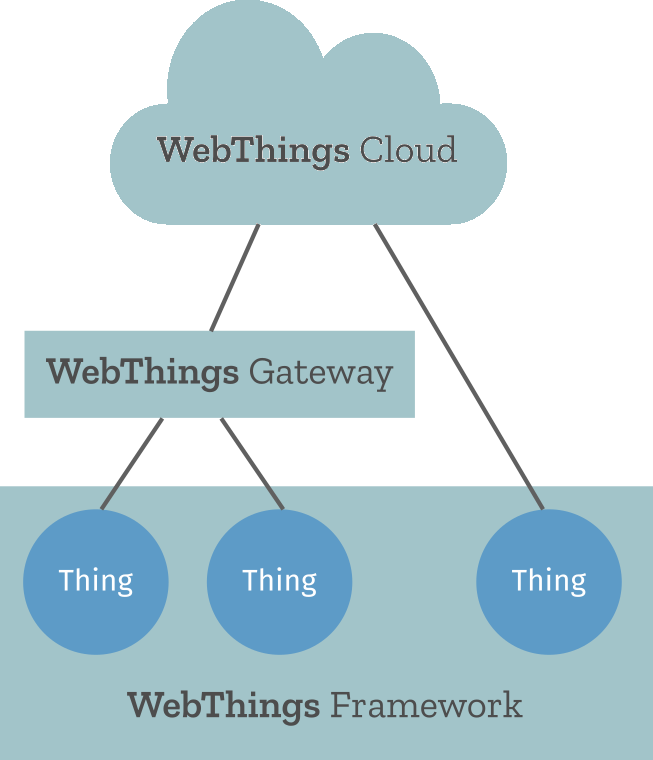
\includegraphics[scale=0.70]{images/webthings/webthings_block_diagram.png}
\caption{Platform overview \cite{wtabout}}
\end{figure}


\subsubsection{Gateway}
WebThings Gateway is the actual platform component through which the users can monitor and control their Smart Home over the web \cite{wtgateway}. It provides:
\begin{itemize}
    \item \textbf{Things UI}: a web user interface (\textbf{\gls{ui}}) to monitor and control the smart home devices.
        \begin{figure}[H]
        \centering
        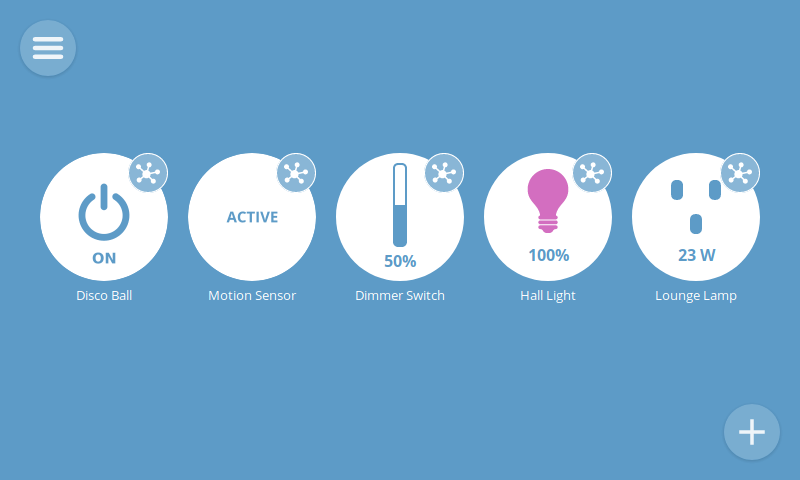
\includegraphics[scale=0.25]{images/webthings/things_ui_screenshot.png}
        \caption{Things UI \cite{wtgateway}}
        \end{figure}

    \item \textbf{Rules Engine}: a simple drag-and-drop interface that provides the ability to to automate the Smart Home devices by creating rules through an ``if this then that'' (\textbf{\gls{ifttt}})\footnote{IFTTT: \href{https://ifttt.com/explore/new_to_ifttt}{ifttt.com}} style (e.g., if it is 7:00 PM, turn the hall light on).
    
        \begin{figure}[H]
        \centering
        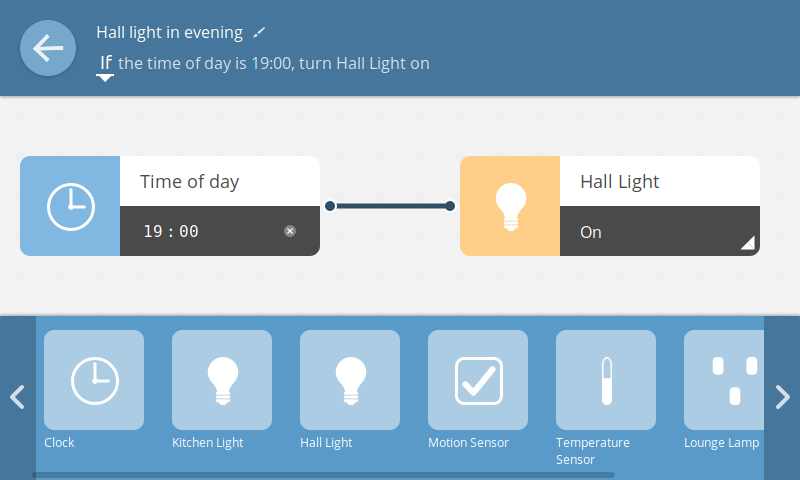
\includegraphics[scale=0.25]{images/webthings/rules_engine_screenshot.png}
        \caption{Rules Engine \cite{wtgateway}}
        \end{figure}

    \item \textbf{Floorplan}: an interactive floorplan of the home on which arrange the devices for a better at-a-glance status and control.
        \begin{figure}[H]
        \centering
        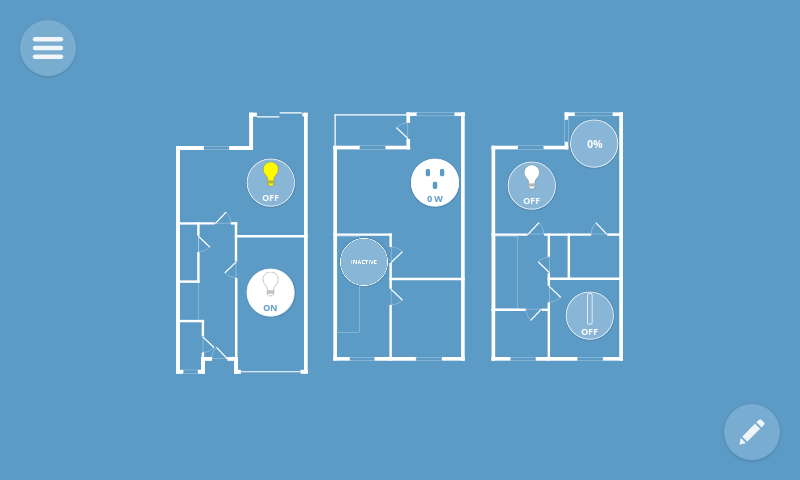
\includegraphics[scale=0.25]{images/webthings/floorplan_screenshot.png}
        \caption{Floorplan \cite{wtgateway}}
        \end{figure}

    \item \textbf{Add-ons}: to extend the Gateway to support a wide range of existing smart home devices and protocols, but also to add new features to the \gls{ui}.
        \begin{figure}[H]
        \centering
        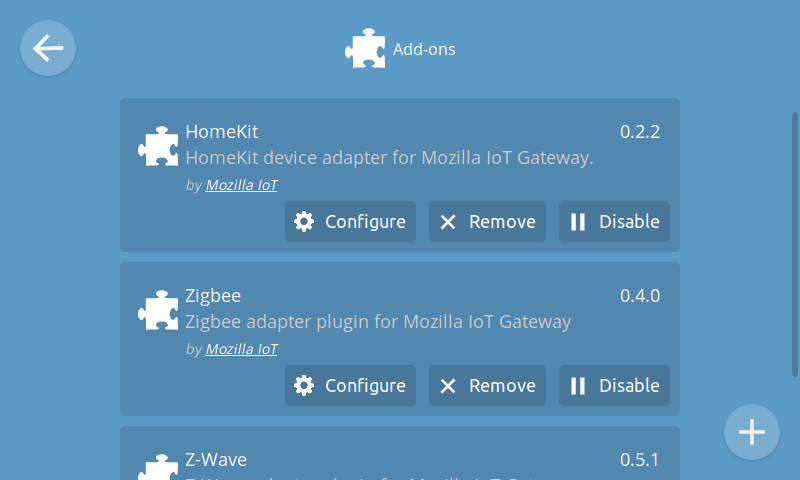
\includegraphics[scale=0.25]{images/webthings/addons_screenshot.png}
        \caption{Add-ons \cite{wtabout}}
        \end{figure}
        
    \end{itemize}


\subsubsection{Framework}
WebThings Framework is a collection of reusable software components to help developers handle their \textbf{\glspl{web thing}} \cite{wtframework}. The framework includes several libraries written in many programming languages, such as \texttt{Node.js}, \texttt{Python}, \texttt{Java}, \texttt{Rust}, \texttt{Arduino}, and \texttt{MicroPython}. Furthermore, the framework also cites third party libraries for other programming languages like \texttt{Go}, \texttt{IoT.js}, \texttt{C\#}, and many more.

\subsubsection{Cloud}
WebThings Cloud provides cloud services for remotely managing the \glspl{web thing} within the Smart Home \cite{wtabout}. Basically, it provides a client with a remote access service to the Smart Home using an end-to-end encrypted 
HTTPS  % https://hacks.mozilla.org/2020/06/mozilla-webthings-gateway-kit-by-okdo/
tunnel between the Gateway and the client.

%    \begin{figure}[H]
%        \centering
%        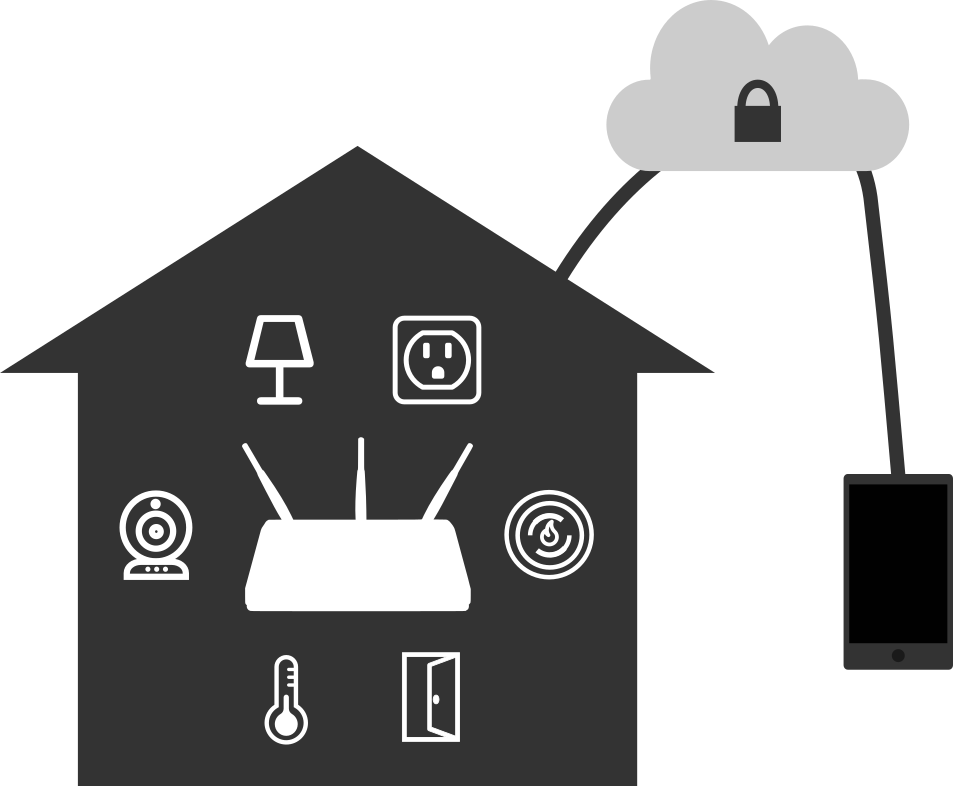
\includegraphics[scale=0.75]{images/webthings/cloud.png}
%        \caption{WebThings Cloud}
%    \end{figure}


\subsection{Gateway Architecture}

The Gateway has two main parts \cite{gatewayarch}: 
\begin{itemize}
    \item The \textbf{back-end} server side: is based on \texttt{\textbf{Node.js}} \cite{nodejshome} and uses \textbf{\texttt{Express} framework} \cite{expressjshome} for routing.
    
    \item The \textbf{front-end} client side: is a single page web application (\textbf{\gls{spa}}), i.e., a web application or website that interacts with the user by dynamically rewriting the current web page with new data from the web server, instead of the default method of a web browser loading entire new pages. Here, routing is controlled via the lightweight  \texttt{\textbf{page.js}} library \cite{pagejsgithub}.
\end{itemize}



\subsubsection{Server Side Components}
The server side, shown in \autoref{gwarch}, can be divided into two main portions.

\begin{figure}[H]
    \centering
    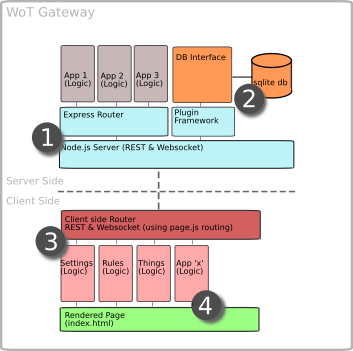
\includegraphics[scale=0.90]{images/webthings/architecture_overview.png}
    \caption{Gateway Architecture Overview \cite{gatewayarch}}
    \label{gwarch}
\end{figure}

In the first portion, when the \verb|Node.js| server starts, the \verb|Express| middleware is bound to the server.
This starting point controls how WebSocket tunnels are created and closed in the Application.

The second server side portion is related to the Gateway's Database. By default, the application uses \texttt{SQLite} \cite{sqlitehome} as a \texttt{SQL} Database Management System (\gls{dbms}).

Lastly, the Gateway logic is based on the Model-View-Controller (\textbf{\gls{mvc}}) paradigm \cite{gamma1993design} (i.e., a software architectural pattern that divides the related program logic into three interconnected elements),
% where 
%\href{https://github.com/WebThingsIO/gateway/tree/master/src/models}
%{\texttt{/src/models}}, 
%\href{https://github.com/WebThingsIO/gateway/tree/master/src/controllers}
%{\texttt{/src/controllers}} and 
%\href{https://github.com/WebThingsIO/gateway/tree/master/src/views}
%{\texttt{/src/views}} contain the relevant MVC's elements for the system
with only one main ``view'' served to the client as a home page.
%which is the 
%\href{https://github.com/WebThingsIO/gateway/blob/master/static/index.html}
%{\texttt{/static/index.html}} file.

\subsubsection{Client Side Components}
Again, keeping \autoref{gwarch} as a reference, it is possible to notice that the Gateway's client side has two main portions too.

Portion three of the client side focuses on routing. In the client, most calls from the main view are interpreted and routed using the \texttt{page.js} library \cite{pagejsgithub}. Then, the router hands off control to the functions designed to handle the specific routes. 
%For example, the \verb|/settings| route is dealt with the
%\href{https://github.com/WebThingsIO/gateway/blob/627c7c401a843c0d2c8418b6d5a40bce98a1e86e/static/js/router.js#L20}
%{\texttt{App.showSettings}}. This uses the \verb|SettingsScreen| module in 
%\href{https://github.com/WebThingsIO/gateway/blob/master/static/js/views/settings.js}
%{\texttt{/static/js/views/settings.js}} to then route calls to the server.

Portion four deals with the rendering of the Gateway's web page.
As already said, the application is based on the \gls{spa} model. Pages are dynamically manipulated in the client side, and changes in the Document Object Model (\textbf{\gls{dom}}) for the main view will be driven by hiding or showing different menu options.
The server supplies data that populates the client.


\subsection{Add-ons}

The WebThings Gateway can be extended with \textbf{add-ons} that, once integrated, provide new features \cite{wtaddonsabout}. Each type of device (or service) needs the proper add-on to be installed and configured so that the Gateway can use it to discover devices and embed them as \glspl{web thing} to interact with.
In WebThings, there are three classes of add-ons: \textit{adapter}, \textit{notifier} and \textit{extension}.

\subsubsection{Adapter add-on}
\label{adapter}

An \textbf{adapter} add-on provides support to the Gateway for some new class of devices (either physical or virtual) by adapting the device into a \gls{web thing}. For instance, a Zigbee \cite{iotzigbee} (i.e., a popular industry wireless mesh networking standard for connecting sensors, instrumentation and control systems \cite{wright2009killerbee}) adapter communicates with Zigbee devices via the Zigbee protocol and represents them as \glspl{web thing} having properties, actions and events.

However, an adapter add-on requires three main components: an adapter object, the device, and  (at least) one property.
\begin{itemize}
    \item The \textbf{adapter object} manages the communication with a device or a set of devices. For example, with all the smart devices using the same protocol for communicating over Wi-Fi.
    \item The \textbf{device} can be physical hardware, such as a smart plug, light bulb, or temperature sensor. Otherwise, it could be a virtual device, such as a weather station providing current weather conditions from a cloud service.
    \item \textbf{Properties} are individual traits of a device, such as its on/off state, its power consumption, or the color of its light.
\end{itemize}


\subsubsection{Notifier add-on}
\label{notifier}

A \textbf{notifier} add-on supplies a new output block for the \gls{rules engine} of the Gateway, allowing a user to be notified of some type of occurrence via some specific mechanism, e.g., e-mail or SMS. A notifier add-on has two primary components: the notifier object and the notification outlet.

\begin{itemize}
    \item A \textbf{notification outlet} is an individual rule output responsible for performing the actual notification process.
    \item A \textbf{notifier} manages a set of notification outlets presented to the user through the \gls{rules interface}. A notifier can own and control any number of outlets.
\end{itemize}


\subsubsection{Extension add-on}
\label{extension}

An \textbf{extension} add-on provides new functionalities to the Gateway's web interface, from something that is purely an aesthetic change (e.g., a new theme), to creating new panels and menu entries that provide new functionalities. An extension add-on has one primary component, an extension object, and an optional API handler.

\begin{itemize}
    \item The \textbf{extension object} is loaded at run-time to provide the desired new functionality.
    \item An \textbf{API handler} is a back-end resource that can extend the Gateway's REST API to provide more functionalities for that specific extension.
\end{itemize}



\section{Threat Modeling}
In Cybersecurity it is important to protect \textbf{assets} from threats. A \textbf{threat} \cite{mayer2007design} is an event that that exploits a \textbf{vulnerability} \cite{mayer2007design}, i.e., a weakness of the asset, and can produce the loss of security properties. An \textbf{attack} \cite{mayer2007design} is a \textit{deliberate} threat occurrence.

The concept of threat modeling is not new. It arose from fields like computer security, cryptography, and risk management many years ago. Threat modeling can be beneficial for any type of system since it involves understanding the complexity of the system and analyzing its representations to highlight concerns about its privacy and security properties giving as output all its possible threats \cite{myagmar2005threat, threatmodelingmanifesto}. An early and frequent analysis is the best way to improve those properties. Threat modeling is also a well-defined approach for identifying and assessing, \textit{proactively}, potential threats and vulnerabilities in systems, applications, and organizations. Hence, having a threat model permits anticipating and mitigating potential risks before a malicious actor can exploit them. With threat modeling, organizations can improve the overall security of their systems by making more thoughtful efforts toward security.

Microsoft
%\footnote{About Microsoft: \href{https://www.microsoft.com/en-us/about}{www.microsoft.com/en-us/about}} 
played an important role in spreading and formalizing threat modeling. In this regard, threat modeling at Microsoft is a documented methodology since 1999 \cite{shostack2008experiences}. Moreover, Microsoft introduced its Security Development Lifecycle (\gls{sdl}), which includes threat modeling, in the early 2000s as an integral part of its software lifecycle, as a key activity to ensure the security of its software products. Since then, many threat modeling methodologies and frameworks have been developed and refined by organizations and security experts. These methodologies typically imply realizing a threat model by looking at the system to assess as an adversary would do. It means looking at the system by identifying its assets, architecture, and potential threats and vulnerabilities. This is done in order to help designers to understand what to asses, but also how and from whom to protect it. 

However, a threat modeling process can be summarized into four main phases \cite{messe2020asset}:
\begin{enumerate}
    \item \textbf{Asset Identification}: it involves identifying security goals, modeling domains, and identifying valuable assets;
    \item \textbf{Threat Enumeration}: it is focused on identifying threats and vulnerabilities. Also, who the possible attackers are and what their motivations are. Lastly, the resulting threats are enumerated and documented;
    \item \textbf{Threat Prioritization}: it involves giving a score to the discovered threats and assessing risks. It is based on the results of the prior phase. This phase can be either considered an internal or external activity \cite{tuma2018};
    \item \textbf{Mitigation}: it aims at resolving threats and lowering the risk level by proposing security mitigations and verifying them.
\end{enumerate}
There is no threat model recommended over another. The decision of which ones to pick should be based on the needs of the project and its specific concerns \cite{shevchenko2018threat}.
A couple of examples of very popular threat models are:
\begin{itemize}
    \item \textbf{STRIDE} \cite{hernan2006threat, shevchenko2018threat, tuma2018two}: its name is an acronym coming from a set of threats, i.e., Spoofing identity, Tampering with data, Repudiation, Information disclosure, Denial of service, and Elevation of privilege \cite{magin2015security}. 
    \begin{itemize}
        \item \textbf{Spoofing}: it happens when there an entity impersonates a different entity;
        
        \item \textbf{Tampering}: it is the unauthorized alteration of data (either in transit or stored);
        
        \item \textbf{Repudiation}: it happens when someone can deny an action after performing it;
        
        \item \textbf{Information disclosure}: it is  the spread of confidential information to unauthorized parties;
        
        \item \textbf{Denial of Service (\gls{dos})}: it is an attack that prevents a system from operating as it should; 
        
        \item \textbf{Elevation of Privilege}: it happens when an entity gets higher system privileges than it should.
        
    \end{itemize}
    It is adopted by Microsoft since 2002. It has a high degree of maturity and evolved to include new threats and new threat enumeration methodologies such as the \textit{STRIDE-per-element} and the \textit{STRIDE-per-interaction}. In particular, the former method is appropriate in systems where each software component to be scanned for potential threats is considered in isolation. The latter method  considers the security threats that might occur in a pair of interacting software components. Hence, it is more appropriate to discover threats in end-to-end scenarios where several components interact.
   
    A STRIDE based threat modeling tool acts in two steps \cite{khan2017stride}. In step one, it takes as input the Data Flow Diagram (\gls{dfd}) of the system and evaluates the system design having the goal of modeling it. Step two consists of the actual threat discovery and analyzing the modeled system. The two STRIDE variants differ in how the exploration of the modeled system is carried out;

    \item \textbf{PASTA} \cite{shevchenko2018threat, ucedavelez2015intro}: it is a risk-centric threat modeling framework focused on attackers' perspective. PASTA is an acronym that stands for Process for Attack Simulation and Threat Analysis. Developed in 2012, it analyzes threats to business logic \cite{kim2022stride} and involves seven stages, i.e., \textit{objectives definition}, \textit{ technical scope definition}, \textit{application decomposition}, \textit{threat analysis}, \textit{vulnerability \& weaknesses analysis}, \textit{attack modeling}, and \textit{risk \& impact analysis}. Each stage uses a variety of design and analysis tools, e.g., \glspl{dfd} are used in the application decomposition stage. In the end, the produced output is an assessment in the form of threat enumeration and scoring.     
\end{itemize}
Hence, threat models can help create realistic and meaningful \textbf{security requirements}, and programmers can take a threat model as a reference to develop something that does not leave open doors for performing system attacks \cite{messe2020asset}. Moreover, a threat model helps to recognize what can go wrong in a system and to point out issues that can influence decisions in the subsequent design, development, testing, and post-deployment stages of the system.
As already said, it is important starting fixing problems in the early stages because the cost of fixing a defect that can be corrected in the requirements stage would increase exponentially in the following phases \cite{lazic2008cost}.

Overall, nowadays threat modeling is an essential practice in the field of cybersecurity and risk management, helping organizations proactively address the security and resilience of their systems and applications.